\documentclass[12pt, titlepage]{article}
\usepackage{graphicx}
\usepackage{booktabs}
\usepackage{hyperref}
\usepackage{tabularx}

\hypersetup{
    colorlinks,
    citecolor=blue,
    filecolor=black,
    linkcolor=red,
    urlcolor=blue
}

\usepackage{color}

\newif\ifcomments\commentstrue

\ifcomments
\newcommand{\authornote}[3]{\textcolor{#1}{[#3 ---#2]}}
\newcommand{\todo}[1]{\textcolor{red}{[TODO: #1]}}
\else
\newcommand{\authornote}[3]{}
\newcommand{\todo}[1]{}
\fi

\newcommand{\wss}[1]{\authornote{blue}{SS}{#1}} 
\newcommand{\plt}[1]{\authornote{magenta}{TPLT}{#1}} %For explanation of the template
\newcommand{\an}[1]{\authornote{cyan}{Author}{#1}}

%% Common Parts

\newcommand{\progname}{ProgName} % PUT YOUR PROGRAM NAME HERE %Every program
                                % should have a name


\begin{document}

\title{System Verification and Validation Plan for Stoichiometry Mass-Mass Program } 
\author{Deemah Alomair}
\date{\today}
	
\maketitle

\pagenumbering{roman}

\section{Revision History}

\begin{tabularx}{\textwidth}{p{3cm}p{2cm}X}
\toprule {\bf Date} & {\bf Version} & {\bf Notes}\\
\midrule
28/10/2019 & 1.0 & First version of document\\
23/12/2019 & 1.0 & Second version of document\\
\bottomrule
\end{tabularx}

\newpage

\tableofcontents

\listoftables 

\listoffigures


\newpage

\section{Symbols, Abbreviations and Acronyms}

\renewcommand{\arraystretch}{1.2}
\begin{tabular}{l l} 
  \toprule		
  \textbf{symbol} & \textbf{description}\\
  \midrule 
   T & Test\\
  SRS & Software Requirements Specification\\
  MIS & Module Interface Specification\\
  MG & Module Guide\\
  SMMP & Stoichiometry Mass-Mass Program \\
  R & Functional requirement\\
  NF & Non-functional requirement\\
  \bottomrule
\end{tabular}\\

\newpage

\pagenumbering{arabic}

\section{General Information}

This document is to build verification and validation plan for Stoichiometry Mass-Mass Program and provide description about the testing that will be carried out on the system. The main goal of this document is to check whether SMMP meets the SRS and fulfill its intended purpose. This document will be used as the reference and guidance for testing SMMP.

\subsection{Summary}

Stoichiometry Mass-Mass Program is a software that convert unbalanced chemical reaction to balanced one. Then do some necessary calculations to get the mass of one of the reactants involved in that chemical reaction.

\subsection{Objectives}

The objectives of the verification and validation plan is to ensure that SMMP is Reliable. Building the confidence of the correctness of the software. In addition, enhance the maintainability for the traceability of the potential changes. Moreover, ensure usability of the SMMP to novel users. 

\subsection{Relevant Documentation}

Relevant Documents that need to be visited while reading this document include the following:
\newline
SRS, which can be found  \href{https://github.com/deemaalomair1/CAS741_project/tree/master/docs/SRS}{SRS} \cite{SoftwareSpecification}
\newline
System Design that includes both MIS and MG, which can be found \href{https://github.com/deemaalomair1/CAS741project/tree/master/docs/Design}{Design} \cite{Designdocument}
\newline
Unit Verification and Validation Plan,  which can be found \href{https://github.com/deemaalomair1/CAS741project/tree/master/docs/VnVPlan/UnitVnVPlan}{UnitVnVPlan} \cite{UnitVnVPlan}
\newline
System and Unit Verification and Validation Report ,  which can be found \href{https://github.com/deemaalomair1/CAS741project/tree/master/docs/VnVReport}{VnVReport} \cite{VnVReport}

\section{Plan}

This section details the plan to be followed when testing the software, including
those involved in the testing, the testing approach, and the verification tools which will be used.
	
\subsection{Verification and Validation Team}

The test team includes the following members:
\begin{itemize}
\item Main contributor: Deemah Alomair.
\item Primary reviewers: Dr. Spencer Smith, Sharon Wu.
\item Secondary reviewers: Bo Cao, Ao Dong, Peter Michalski.
\end{itemize}

\subsection{SRS Verification Plan}

\begin{itemize}
\item  Feedback: Classmates, including all primary and secondary reviewers
listed above, will provide feedback on GitHub by submitting an issue in the
issue tracker. They will read the document and provide a guidelines on how to enhance the document.
\item Initial Review: The document will be manually reviewed by Dr. Spencer Smith
using the SRS checklist upon its initial creation, as found in the CAS741
GitLab repository 
\end{itemize}

\subsection{Design Verification Plan}

\begin{itemize}
\item  Feedback: Classmates, including all primary and secondary reviewers
listed above, will provide feedback on GitHub by submitting an issue in the
issue tracker. They will read the document and provide a guidelines on how to enhance the document.
\item Initial Review: The documents will be manually reviewed by Dr. Spencer Smith
using the MG/MIS checklists upon its initial creation, as found in the CAS741
GitLab repository 
\end{itemize}

\subsection{Implementation Verification Plan}

Implementation Verification Plan will include the followings:
\begin{itemize}
\item Manual testing.
\item  Automatic testing that includes unit testing for each individual function and coverage testing using "unittest package" and "coverage package" that work with PyCharm environment.
\item Parallel testing. 
\end{itemize}

\subsection{Software Validation Plan}

The main goal of this project is to build the product right and get a correct calculated output. 
As the developer and the user is the same person software validation plan is not applicable.

\section{System Test Description}

This section lists the system tests to be performed to verify whether or not the
program fulfills the functional requirements and to test how well it meets the
non-functional requirements. Note that some of the tests for the functional
requirements are unit tests.

\subsection{Tests for Functional Requirements}


\subsubsection{Input Tests}

		
\paragraph{Input conversion tests}

\begin{enumerate}

\item{MassInputTest-id1\\}

Control: Functional, dynamic, automatic.
					
Initial State: Not Applicable.
					
Input: 
\begin{table}[h!]
\centering
\begin{tabular}{|c|c|}
\hline
input & response  \\
\hline
Mass $\notin$ number  & error massage \\ \hline
Mass $\leq$ 0& error massage \\ \hline
Mass $>$ 0  & accepted\\ \hline
\hline
\end{tabular}
\caption{Input possible value's level }
\label{tab:reqtrace}
\end{table}

					
Output: error massage indicating that mass value is not a number or mass value $\leq$ 0. 

Test Case Derivation: the expected value is a positive integer number. 
					
How test will be performed: 
\begin{itemize}
\item the system will get the value. 
\item process the value to ensure it's a number. if not error massage will be shown.
\item if its a number it will test if its greater than 0 or not.  if not error massage will be shown.
\end{itemize}



\item{ReactionInputTest-id2\\}

Control: Functional, dynamic, automatic.
					
Initial State: Not Applicable
					
Input: 
1. reaction element = selection from drop down menu.
\newline
2. atom value: 
\begin{table}[h!]
\centering
\begin{tabular}{|c|c|}
\hline
atom value & response  \\
\hline
atom value $\notin$ number  & error massage \\ \hline
atom value $\leq$ 0& error massage \\ \hline
atom value $>$ 0  & accepted\\ \hline
\hline
\end{tabular}
\caption{Input possible value's level }
\label{tab:reqtrace}
\end{table}
	
Output: error massage indicating that atom value is not a number or atom value $\leq$ 0. 

Test Case Derivation: the expected value is chemical element selected from a menu and atom value belongs to positive integer number. 

How test will be performed: 
\begin{itemize}
\item the system will get the values. 
\item the system will ensure user has already selected an element. 
\item process the atom value to ensure it's a number. if not error massage will be shown.
\item if its a number it will test if its greater than 0 or not.  if not error massage will be shown.
\end{itemize}


\end{enumerate}					

\subsubsection{Output Tests}

\paragraph{Output constrains tests}
throughout the rest of this document we will use one chemical reaction as an example. in real testing we can use different chemical reactions as long as it consists of two reactants, each consists of two element at most.
reaction used : ”$Fe_2$$O_3$ + C $\rightarrow$ Fe + C$O_2$”. 

\begin{enumerate}

\item{ReactionOutputTest-id3\\}

Control: Functional, dynamic, automatic.
					
Initial State: N.A
					
Input: 
chemical reaction : ”$Fe_2$$O_3$ + C $\rightarrow$ Fe + C$O_2$”
two reactants and two products each with maximum two elements.
	
Output: balance reaction : 2$Fe_2$$O_3$ + 3C $\rightarrow$ 4Fe + 3C$O_2$

Test Case Derivation: the expected value is balance chemical reaction by adding the appropriate coefficients in front of each reactant and product.

How test will be performed: 
\begin{itemize}
\item the system will get chemical reaction elements and atoms value. 
\item if the entered reaction is not balance then the system will output the balanced reaction instead. 
\item the balance result will be compared to \cite{OnlineBalancer} as parallel testing.
\end{itemize}


\item{MassOutputTest-id4\\}

Control: Functional, dynamic, automatic.
					
Initial State: Not Applicable
					
Input:
\newline
chemical reaction : ”$Fe_2$$O_3$ + C $\rightarrow$ Fe + C$O_2$”
\newline
mass of known reactant : 2
\newline
name of known reactant: ”$Fe_2$$O_3$”
				
Output: C mass = 0.1 g. 

Test Case Derivation: the expected value is a positive integer number. 
					
How test will be performed: 
the system will calculate mass value using the calculation method and ensure it's greater than 0.
 


\end{enumerate}	

\subsubsection{Calculation Method Tests}

\begin{enumerate}

\item{CheckBalanceTest-id5\\}

Control: Functional, dynamic, automatic.
					
Initial State: N.A
					
Input: 
\newline
chemical reaction : ”$Fe_2$$O_3$ + C $\rightarrow$ Fe + $CO_2$”
two reactants and two products each with maximum two elements.
	
Output: "not balance !"

Test Case Derivation: the expected value is balance when chemical reaction is balance and not balance otherwise. 

How test will be performed: 
\begin{itemize}
\item the system will get chemical reaction elements and atoms value. 
\item the system will calculate the total atom value for each element in each side of the reaction. 
\item the system will compare the total of each element in both side and repeat this process for each element involved in the reaction.
\item if total atoms value in reactant side = total atoms value in product side then the chemical reaction considered balance .
\item "balance" will be displayed to the user using GUI widget. 
\item if not balance then balance form will be calculated and "not balance !" will be displayed to the user using GUI widget with the new form of the reaction.
\end{itemize}

more tests will be performed on balancing chemical reaction as unit testing in unit testing plan. \cite{UnitVnVPlan}

\item{MolecularWeightCalculationTest-id6\\}

Control: Functional, dynamic, automatic.
					
Initial State: Not Applicable
					
Input: name of known reactant: ”$Fe_2$$O_3$”
				
Output:  Molecular weight = 55.845*2 + 15.9994*3 =  159.6882 g/mol. 

Test Case Derivation: the expected value is a molecular weight which is equal to the sum of  atomic mass multiplied by the total atom value for each element building up the reactant. 
					
How test will be performed: 
\begin{itemize}
\item the system will get the atomic mass for each element of the reactant.
\item multiply each atomic mass by the total atoms of the element 
\item add the result of each element together.
\item save the final result to be used in other function.
\end{itemize}

\item{Mole1CalculationTest-id7\\}

Control: Functional, dynamic, automatic.
					
Initial State: Not Applicable
					
Input: Mass = 2 g , molecular weight = 159.6882 g/mol
			
Output:  Mole = 2 / 159.6882 =  0.0125 mol. 

Test Case Derivation: the expected value is mole for reactant with known mass which is equal to given mass value divided by calculated molecular weight. 	
				
How test will be performed: 
\begin{itemize}
\item the system will get mass and molecular weight  for the reactant.
\item divide mass by molecular weight 
\item save the final result to be used in other function.
\end{itemize}

\item{MoleRatioCalculationTest-id8\\}

Control: Functional, dynamic, automatic.
					
Initial State: Not Applicable
					
Input: coefficient1 = 2  , coefficient2 = 3
			
Output:  coefficient2/coefficient1 = 3/2 = 1.5 

Test Case Derivation: the expected value is Mole Ratio which is equal to derived coefficient value of reactant with unknown mass divided by coefficient value of reactant with known mass.
 					
How test will be performed: 
\begin{itemize}
\item the system will get coefficient2 and coefficient1 derived from balancing the reaction..
\item divide coefficient2 by coefficient1  
\item save the final result to be used in other function.
\end{itemize}

\item{Mole2CalculationTest-id9\\}

Control: Functional, dynamic, automatic.
					
Initial State: Not Applicable
					
Input: Mole1 = 0.0125  , MoleRatio = 1.5
			
Output:  Mole1/MoleRatio = 0.0125/1.5 =  0.008

Test Case Derivation: the expected value is Mole2 (mole for reactant with unknown mass ) which is equal to Mole1 value divided by MoleRatio.  				
	
How test will be performed: 
\begin{itemize}
\item the system will get Mole1 and MoleRatio derived from other functions
\item divide Mole1 by MoleRatio  
\item save the final result to be used in other function.
\end{itemize}

\item{MassCalculationTest-id10\\}

Control: Functional, dynamic, automatic.
					
Initial State: Not Applicable
					
Input: Mole2 = 0.0062  , Molecular weight = 12.0107
			
Output:  Mole2 * Molecular weight = 0.008 * 12.0107 = 0.1 g.

Test Case Derivation: the expected value is final Mass which is equal to Mole2 value multiplied by reactant Molecular weight.  				

How test will be performed: 
\begin{itemize}
\item the system will get Mole2 and Molecular weight derived from other functions
\item multiply Mole2 by Molecular weight  
\item send the final result to GUI to be displayed.
\end{itemize}

\end{enumerate}		
	
\subsection{Tests for Nonfunctional Requirements}

\begin{enumerate}

\item{ UsabilityTesting-id11\\}

Type:  Nonfunctional,Dynamic, Manual.
					
Initial State:  Not Applicable.
					
Input/Condition: chemical reaction ,  mass of one reactant
					
Output/Result: Balance reaction , Second reactant mass.
					
How test will be performed: user need to complete small survey. see appendix A 
					
\item{Reliability-id12\\}

Type: Functional, Dynamic, Manual, Static etc.
					
Initial State:  Not Applicable.
					
Input: testing 25 unbalanced chemical reaction with given mass for one reactant.
					
Output: the percentage of correct answer. (aim for 100 \% correct answer) 
					
How test will be performed: the developer manually will test the overall system using 25 different examples of unbalanced chemical reaction consists of two reactant each consist of at most two elements with given mass of one of reactant, and get the percentage of correct answer. correct answer will include: (right balancing + correct mass value) 

\end{enumerate}

\subsection{Traceability Between Test Cases and Requirements}

A trace between system tests and requirements is provided in 
\hyperref[tab:reqtrace]{Table~\ref*{tab:reqtrace}}.

\begin{table}[h!]
\centering
\begin{tabular}{|c|c|c|c|c|c|c|c|c|c|c|c|c|c|}
\hline
	& T1 & T2 & T3 & T4 & T5 & T6 & T7 &T8  & T9 & T10 & T11 & T12  \\
\hline
R1  & X& X& & & & & & &  & & &  \\ \hline
R2  & & & X& X& & & & &  & & &  \\ \hline
R3  & & & & &X &X&X & X &X &X & &  \\ \hline
R4  &X & X& X& X&X &X&X & X & X& X& & \\ \hline
NF1 & & & & & & & & &  & &X &  \\ \hline
NF2   & & & & & & & & &  & & & X  \\ \hline
\hline
\end{tabular}
\caption{Traceability Matrix Showing the Connections Between Requirements and system tests}
\label{tab:reqtrace}
\end{table}
\newpage
\bibliographystyle{unsrt}

\bibliography{../../refs/References}

\newpage

\section{Appendix}
 \begin{figure}[h!]
 \begin{center}
 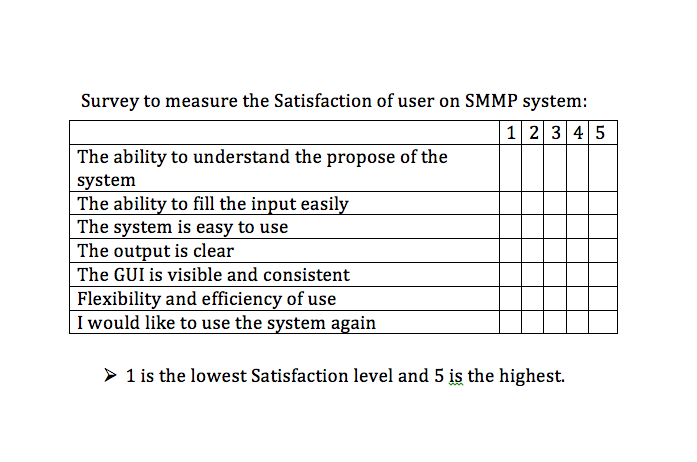
\includegraphics [width=\textwidth]{survey}
 \caption{\label{ Figure 1:} user satisfaction survey.}
 \end{center}
 \end{figure}


\end{document}
